\subsubsection{\textit{Authentication service}}

El \textit{authentication service} es el encargado de la gestión de usuarios y asegura la autenticación de los mismos.
Las principales funcionalidades que ofrece este servicio son: el registro de usuarios, la autenticación y autorización de
los mismos, así como también el control de tokens de acceso, en lo referente a su expiración y validez. También permite
que los usuarios puedan recuperar sus contraseñas.
\vspace{0.25cm}

Los usuarios de nuestra aplicación presentan dos niveles o tipos de autorización: usuarios o \textit{players} y
administradores. Los usuarios tienen acceso a la mayoría de los \textit{endpoints}, excepto a los relacionados con
cuestiones específicas, mientras que los administradores pueden acceder a todos los \textit{endpoints}.
\vspace{0.25cm}

La información requerida para cada usuario es el email para identificarlos de forma unívoca y enviarles correos
electrónicos, y la contraseña como método de autenticación. Además, se diferencia con un valor \textit{booleano} si un
usuario es un \textit{player} o un administrador.
\vspace{0.25cm}

El flujo de registro para un \textit{player} consiste en enviar una petición a \texttt{POST /auth/signup}, donde facilita su
email y su contraseña. La contraseña requiere un mínimo de 8 caracteres y debe contener al menos un número y una letra.
A continuación se le envía un código por correo para verificar su identidad; dicho código tiene una longitud de 8 caracteres 
alfanuméricos.
\vspace{0.25cm}

\begin{figure}[h]
    \centering
    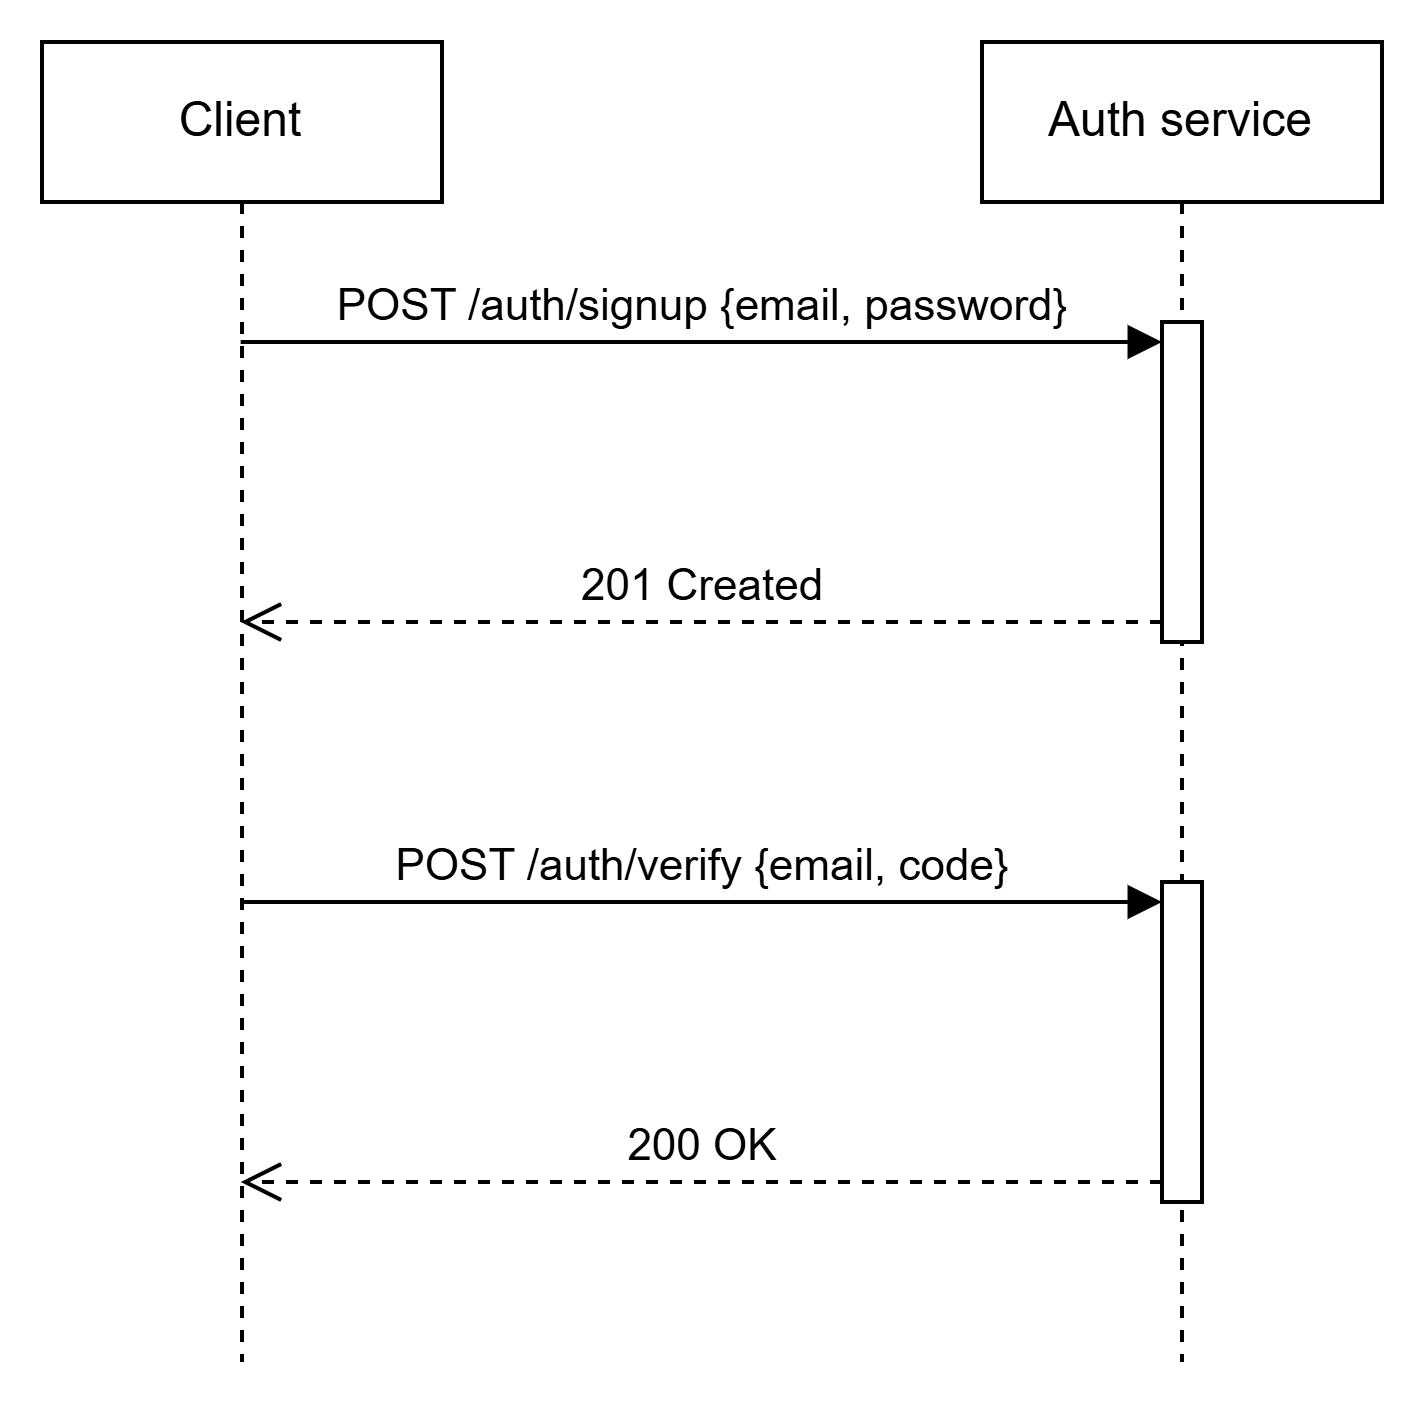
\includegraphics[width=0.55\textwidth]{img/08-implemented-solution/core-service/auth-service-case-1.png}
    \caption{Diagrama de secuencia del flujo de registro}
    \label{fig:auth-service-case-1}
\end{figure}

La verificación se realiza mediante \texttt{POST /auth/verify}, y el código se puede regenerar con 
\texttt{POST /auth/refresh}. La petición de verificación requiere enviar también el correo; se disponen de hasta tres 
intentos para verificar el código. Si se fallan los tres intentos, la cuenta queda en un estado inválido que impide volver 
a registrarse.
\vspace{0.25cm}

Posteriormente, se debe enviar una petición a \texttt{POST /auth/login}. Con esa petición se reciben los tokens de
acceso (\textit{access tokens}) para acceder a los \textit{endpoints} restringidos o que requieren autenticación. Los
tokens son \textit{JSON Web Tokens} (JWT), los cuales almacenan información relevante de la sesión, como el ID del
usuario y la fecha de expiración. La duración de estos tokens es de 1 día.
\vspace{0.25cm}

En caso de que la sesión venza, existe la posibilidad de regenerar el token mediante los tokens de refresco
(\textit{refresh tokens}), que tienen un vencimiento de 30 días. Para comprobar el estado de una sesión existe el
\textit{endpoint} \texttt{GET /auth/check-session}, que retorna el estado de la sesión; para regenerar los tokens se
utiliza \texttt{POST /auth/refresh-token}, que regenera el \textit{access token} y el \textit{refresh token}. 
\vspace{0.25cm}

Además, se actualiza en la tabla de usuarios la fecha de creación del último \textit{refresh token} para invalidar todos 
los tokens anteriores en caso de que el usuario haya sufrido un ataque de \textit{sniffing} de paquetes a través de un
"Man-in-the-Middle". De este modo, un usuario deberá volver a autenticarse solo si permanece 30 días seguidos inactivo.
\vspace{0.25cm}

El flujo de recuperación de contraseña consta de tres pasos. En primer lugar, el usuario envía una petición a
\texttt{POST /auth/password/forgot} con su dirección de correo electrónico. En caso de que el correo corresponda a una 
cuenta registrada, se genera un código OTP (\textit{One-Time Password}) y se envía al correo del usuario.
\vspace{0.25cm}

\begin{figure}[h]
    \centering
    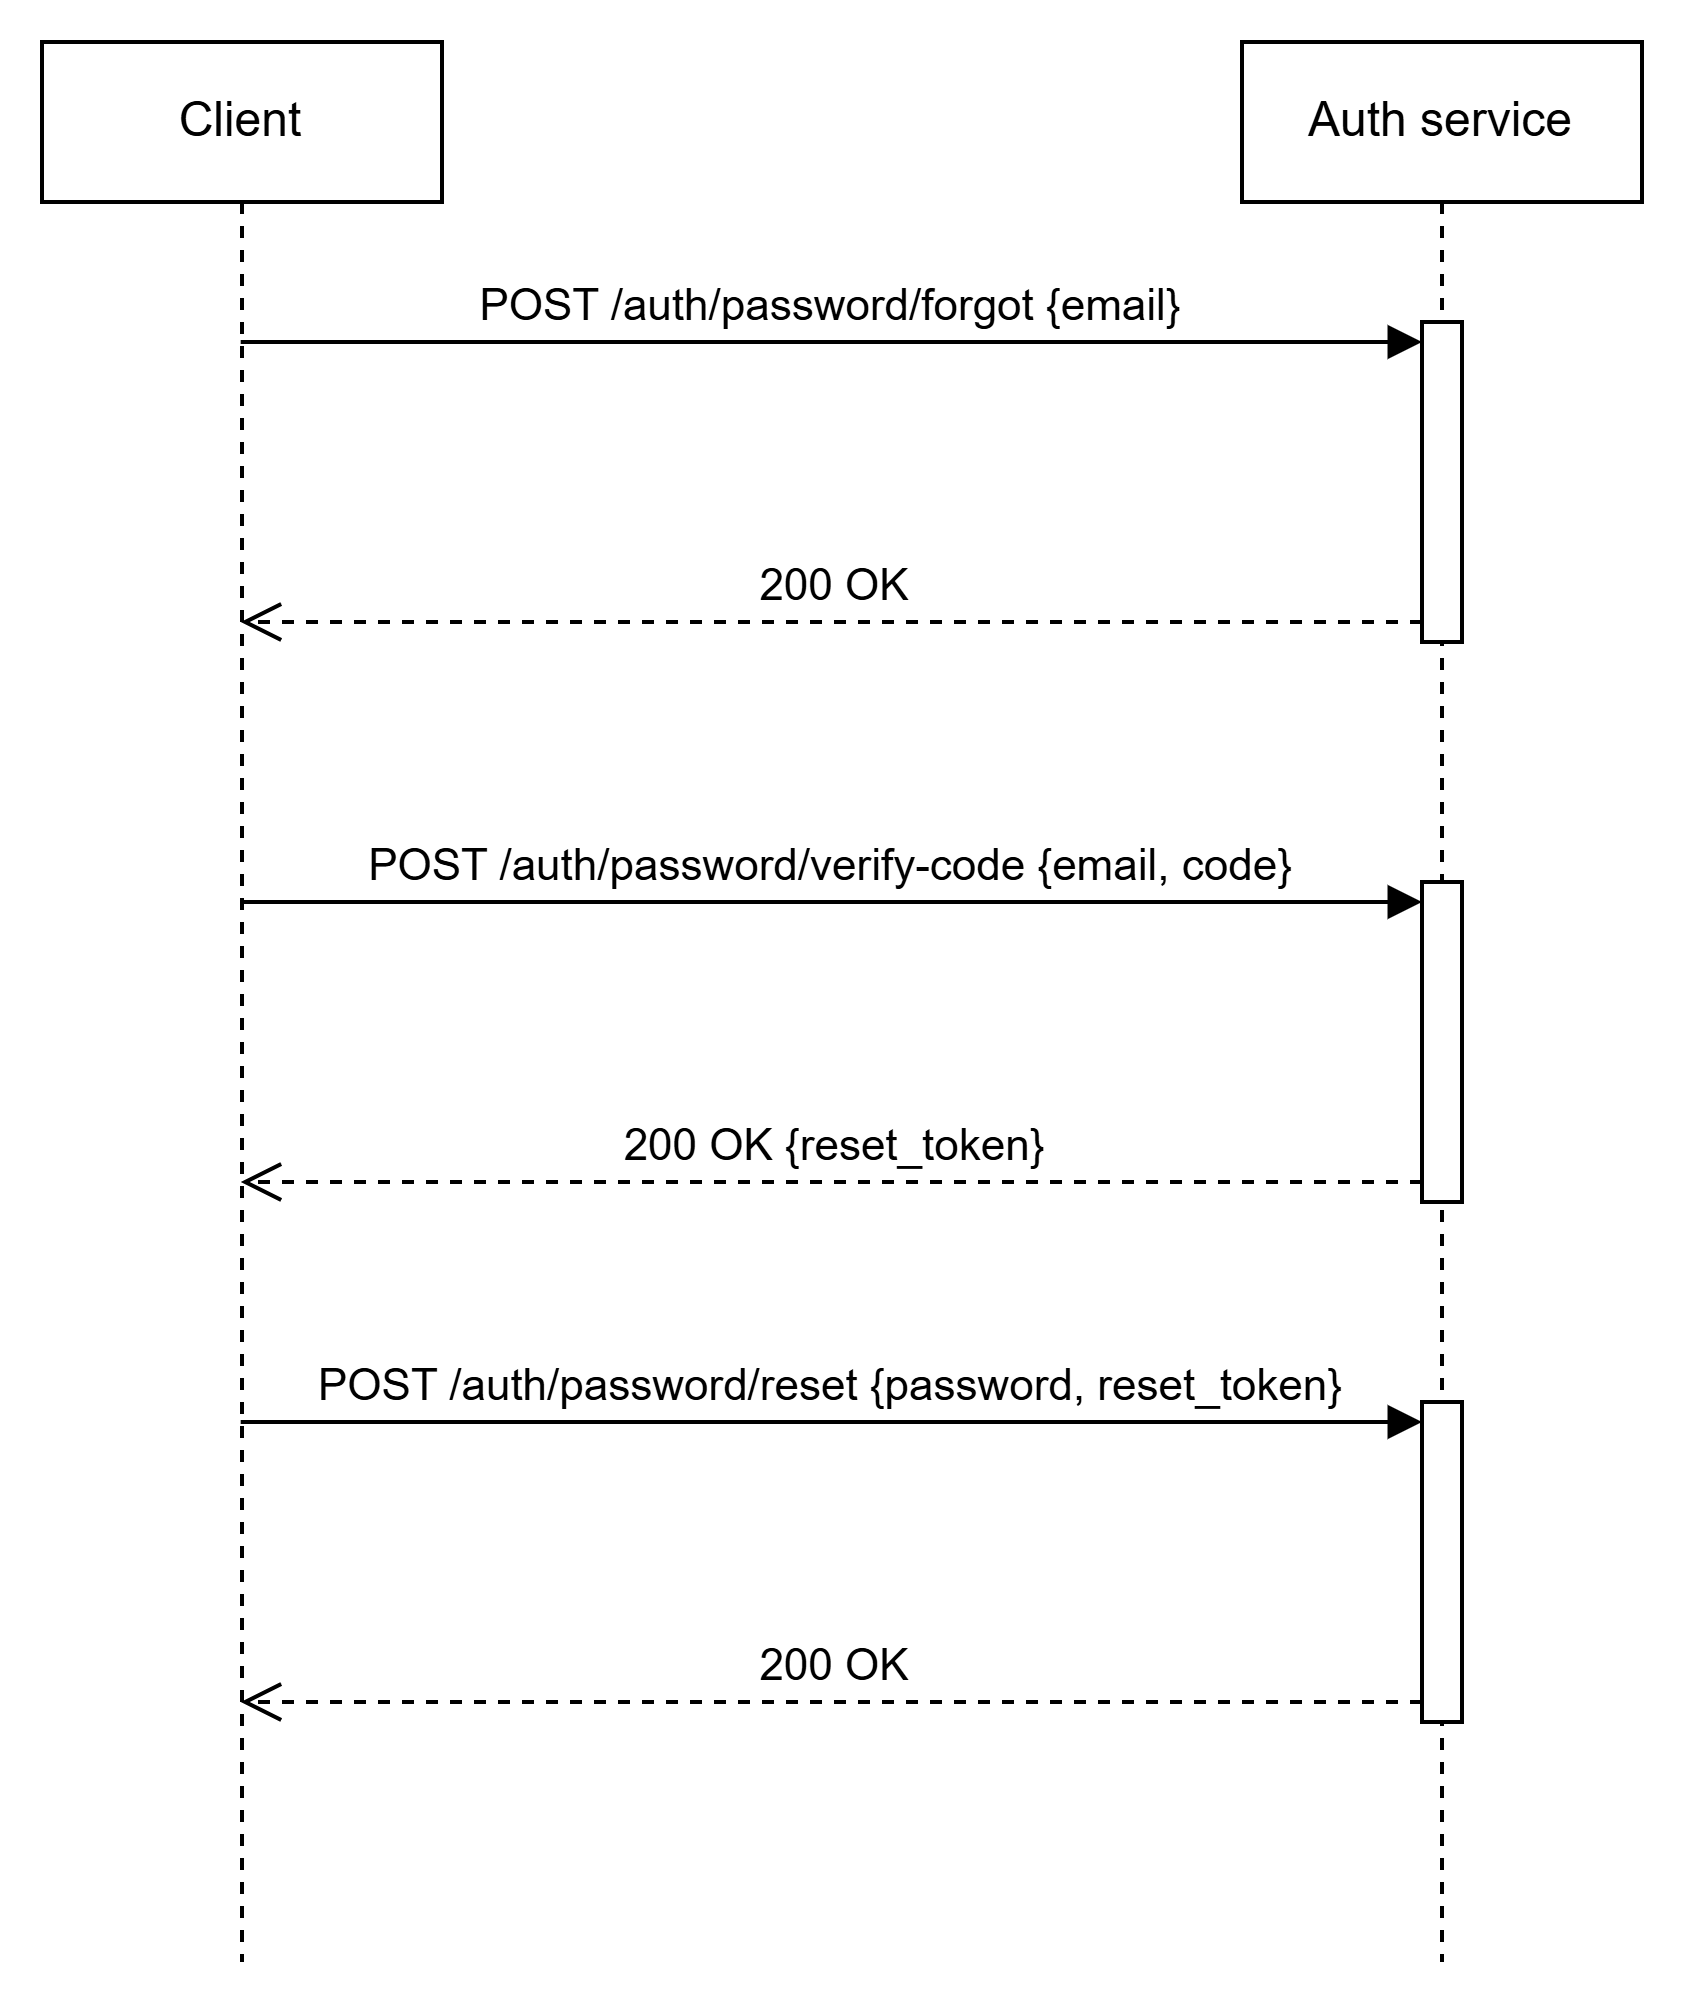
\includegraphics[width=0.65\textwidth]{img/08-implemented-solution/core-service/auth-service-case-2.png}
    \caption{Diagrama de secuencia del recuepero de contraseña}
    \label{fig:auth-service-case-2}
\end{figure}

A continuación, el usuario debe verificar el código recibido mediante el \textit{endpoint} \texttt{POST /auth/password/verify-code},
proporcionando su correo y el OTP. El sistema contempla distintas casuísticas de error, como código incorrecto,
código expirado o número máximo de intentos superado. Si el código es válido, se emite un token de restablecimiento
(\textit{reset token}) de corta duración. Y usuario completa el proceso enviando el \textit{reset token} junto con la 
nueva contraseña a \texttt{POST /auth/password/reset}. 
\vspace{0.25cm}

El sistema valida el token, comprueba que la contraseña cumpla el formato requerido y, de ser así, actualiza las credenciales 
e invalida todas las sesiones activas del usuario. Si el token ha expirado o ya fue utilizado, el usuario deberá iniciar 
el flujo desde el principio.
\vspace{0.25cm}

\newpage

\underline{\textbf{Endpoints}}

\renewcommand{\arraystretch}{1.4}
\begin{longtable}{|l|l|p{7cm}|}
\hline
\textbf{Verbo HTTP} & \textbf{Path} & \textbf{Descripción} \\
\hline
\endfirsthead

\hline
\textbf{Verbo HTTP} & \textbf{Path} & \textbf{Descripción} \\
\hline
\endhead

\endfoot

\texttt{POST} & \texttt{/auth/signup}               & Crea una nueva cuenta de usuario con email y contraseña. \\
\hline
\texttt{POST} & \texttt{/auth/login}                & Autentica a un usuario y retorna un access token y refresh token. \\
\hline
\texttt{GET}  & \texttt{/auth/check-session}        & Valida la integridad y expiración del token activo. \\
\hline
\texttt{GET}  & \texttt{/auth/session}              & Verifica que la sesión activa tenga privilegios de administrador. \\
\hline
\texttt{POST} & \texttt{/auth/verify}               & Verifica el email del usuario con el código de verificación recibido. \\
\hline
\texttt{POST} & \texttt{/auth/refresh}              & Genera y envía un nuevo código de verificación al email del usuario. \\
\hline
\texttt{POST} & \texttt{/auth/password/forgot}      & Inicia el flujo de recuperación de contraseña enviando un OTP al email. \\
\hline
\texttt{POST} & \texttt{/auth/password/verify-code} & Valida el OTP enviado al email y retorna un token de reset de vida corta. \\
\hline
\texttt{POST} & \texttt{/auth/password/reset}       & Valida el token de reset y actualiza la contraseña, revocando todas las sesiones activas. \\
\hline
\texttt{POST} & \texttt{/auth/refresh-token}        & Valida el refresh token y emite un nuevo par de access token y refresh token. \\
\hline
\texttt{GET}  & \texttt{/auth/users}                & Retorna una lista paginada de usuarios. Solo administradores. \\
\hline
\texttt{PUT}  & \texttt{/auth/users/\{id\}/admin}   & Actualiza el estado de administrador de un usuario. Solo administradores. \\
\hline
\caption{\textit{Endpoints} del \textit{authentication service}}
\label{tab:auth-endpoints}
\end{longtable}

\underline{\textbf{Tablas de \textit{authentication service}}}
\vspace{0.25cm}

\underline{\textbf{Tabla \texttt{users}}}

\renewcommand{\arraystretch}{1.4}
\begin{longtable}{|l|l|p{7cm}|}
\hline
\textbf{Columna} & \textbf{Tipo} & \textbf{Descripción} \\
\hline
\endfirsthead
\hline
\textbf{Columna} & \textbf{Tipo} & \textbf{Descripción} \\
\hline
\endhead
\endfoot

\texttt{id}                         & \texttt{UUID}         & Clave primaria. Generado automáticamente con \texttt{gen\_random\_uuid()}. \\
\hline
\texttt{email}                      & \texttt{TEXT}         & Dirección de correo electrónico. Debe ser única en la tabla. \\
\hline
\texttt{password}                   & \texttt{TEXT}         & Contraseña almacenada hasheada. \\
\hline
\texttt{verified}                   & \texttt{BOOLEAN}      & Indica si la cuenta fue verificada. Por defecto: \texttt{FALSE}. \\
\hline
\texttt{is\_admin}                  & \texttt{BOOLEAN}      & Indica si el usuario tiene privilegios de administrador. Por defecto: \texttt{FALSE}. \\
\hline
\texttt{refresh\_token\_updated\_at} & \texttt{TIMESTAMPTZ} & Marca temporal de la última actualización del refresh token. \\
\hline
\texttt{created\_at}                & \texttt{TIMESTAMPTZ}  & Fecha y hora de creación del registro. Por defecto: \texttt{now()}. \\
\hline
\texttt{updated\_at}                & \texttt{TIMESTAMPTZ}  & Fecha y hora de última actualización. Por defecto: \texttt{now()}. \\
\hline
\caption{Tabla \texttt{users} del \textit{authentication service}}
\label{tab:users}
\end{longtable}

\vspace{1em}
\underline{\textbf{Tabla \texttt{account\_verifications}}}

\renewcommand{\arraystretch}{1.4}
\begin{longtable}{|l|l|p{7cm}|}
\hline
\textbf{Columna} & \textbf{Tipo} & \textbf{Descripción} \\
\hline
\endfirsthead
\hline
\textbf{Columna} & \textbf{Tipo} & \textbf{Descripción} \\
\hline
\endhead
\endfoot

\texttt{user\_id}           & \texttt{UUID}      & Clave primaria y clave foránea hacia \texttt{users(id)}. \\
\hline
\texttt{verification\_code} & \texttt{TEXT}      & Código de verificación enviado al usuario. Por defecto: cadena vacía. \\
\hline
\texttt{attempts}           & \texttt{INTEGER}   & Número de intentos de verificación realizados. Por defecto: \texttt{0}. \\
\hline
\texttt{created\_at}        & \texttt{TIMESTAMP} & Fecha y hora de creación del registro. Por defecto: \texttt{NOW()}. \\
\hline
\texttt{expires\_at}        & \texttt{TIMESTAMP} & Fecha y hora de expiración del código. Por defecto: \texttt{NOW() + 10 minutos}. \\
\hline
\caption{Tabla \texttt{account\_verifications} del \textit{authentication service}}
\label{tab:account-verifications}
\end{longtable}

\vspace{1em}
\underline{\textbf{Tabla \texttt{password\_resets}}}

\renewcommand{\arraystretch}{1.4}
\begin{longtable}{|l|l|p{7cm}|}
\hline
\textbf{Columna} & \textbf{Tipo} & \textbf{Descripción} \\
\hline
\endfirsthead
\hline
\textbf{Columna} & \textbf{Tipo} & \textbf{Descripción} \\
\hline
\endhead
\endfoot

\texttt{id}                        & \texttt{UUID}         & Clave primaria. Generado con \texttt{gen\_random\_uuid()}. \\
\hline
\texttt{user\_id}                  & \texttt{UUID}         & Clave foránea hacia \texttt{users(id)}. Indexada. \\
\hline
\texttt{otp\_hash}                 & \texttt{TEXT}         & Hash del OTP enviado al usuario por correo electrónico. \\
\hline
\texttt{reset\_token\_hash}        & \texttt{TEXT}         & Hash del token de reset, emitido tras validar el OTP. Indexado. \\
\hline
\texttt{attempts}                  & \texttt{INTEGER}      & Número de intentos de ingreso del OTP. Por defecto: \texttt{0}. \\
\hline
\texttt{otp\_expires\_at}          & \texttt{TIMESTAMPTZ}  & Fecha y hora de expiración del OTP. \\
\hline
\texttt{reset\_token\_expires\_at} & \texttt{TIMESTAMPTZ}  & Fecha y hora de expiración del token de reset. \\
\hline
\texttt{otp\_verified}             & \texttt{BOOLEAN}      & Indica si el OTP fue validado exitosamente. Por defecto: \texttt{FALSE}. \\
\hline
\texttt{used}                      & \texttt{BOOLEAN}      & Indica si el registro ya fue utilizado para resetear la contraseña. Por defecto: \texttt{FALSE}. \\
\hline
\texttt{created\_at}               & \texttt{TIMESTAMPTZ}  & Fecha y hora de creación del registro. Por defecto: \texttt{NOW()}. \\
\hline
\caption{Tabla \texttt{password\_resets} del \textit{authentication service}}
\label{tab:password-resets}
\end{longtable}

\vspace{1em}
Tanto \texttt{account\_verifications} como \texttt{password\_resets} referencian a \texttt{users} mediante \texttt{FOREIGN KEY} 
con \texttt{ON DELETE CASCADE}, de modo que al eliminar un usuario se eliminan en cascada todos sus registros de verificación 
y de restablecimiento de contraseña.
